





\subsection{Test with $M=N$ on EEG Data Set, For Reference}
\begin{itemize}
\item here we have pair each couple of row with the lowest MSE, because ICA do not localize the sources in the same manner.
\end{itemize}

\begin{figure}[H]
    \centering
	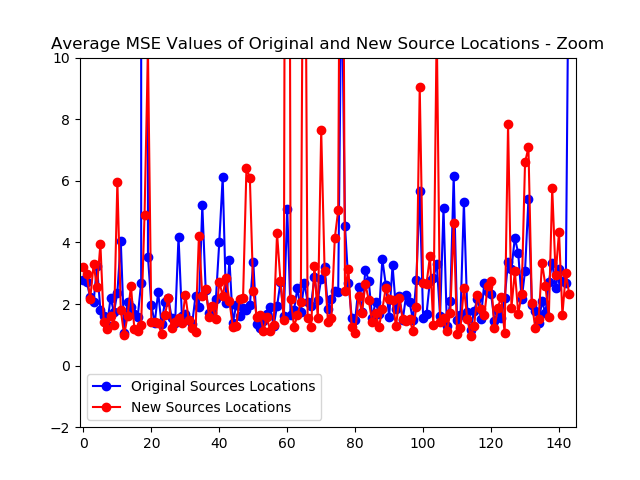
\includegraphics[scale=0.5]{figures/ch_7/M=N_1.png}
	\caption{MSE for system with M=N}
	\label{fig:M=N_1}
\end{figure}  

\begin{figure}[H]
    \centering
	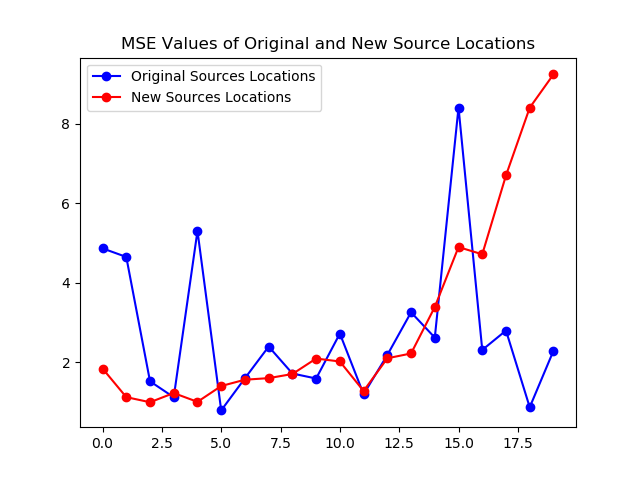
\includegraphics[scale=0.5]{figures/ch_7/M=N_3.png}
	\caption{MSE for system with M=N}
	\label{fig:M=N_3}
\end{figure} 

\begin{figure}[H]
    \centering
	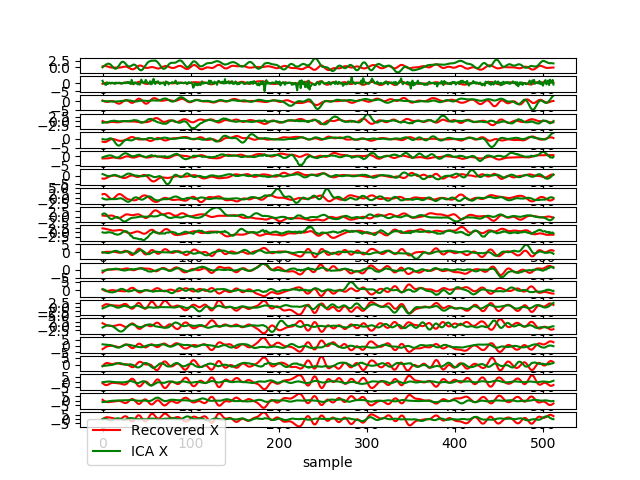
\includegraphics[scale=0.5]{figures/ch_7/M=N_2.png}
	\caption{example of one segment of the system with $M=N$}
	\label{fig:M=N_2}
\end{figure} 

\begin{itemize}
\item plot \ref{fig:M=N_1} is the case of $N=M$, is to be use as a reference, as that is the 'best' we can archieve.
\item plot \ref{fig:M=N_3} is MSE of each row, in one segment. 
\item plot \ref{fig:M=N_2} is the MSE for every segment, this is to be compared the first plot.
 
\item plot \ref{fig:M=N_test} show that our algorithm can manage to find the almost exact solution in this 'easy' case $N=M$ 
\end{itemize}

\begin{figure}[H]
    \centering
	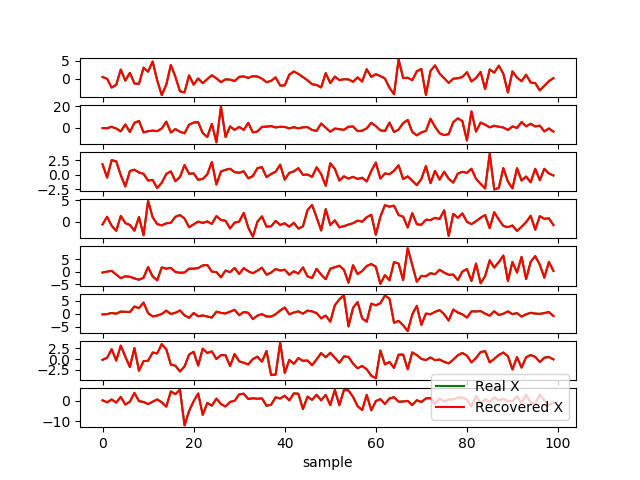
\includegraphics[scale=0.5]{figures/ch_7/M=N_test.png}
	\caption{example to varify tht our system gets the exact result for M=N, MSE is 3.78e-28 }
	\label{fig:M=N_test}
\end{figure}





\subsection{Test with $\frac{1}{3} M<N$ on EEG Data Set}
\begin{figure}[H]
    \centering
	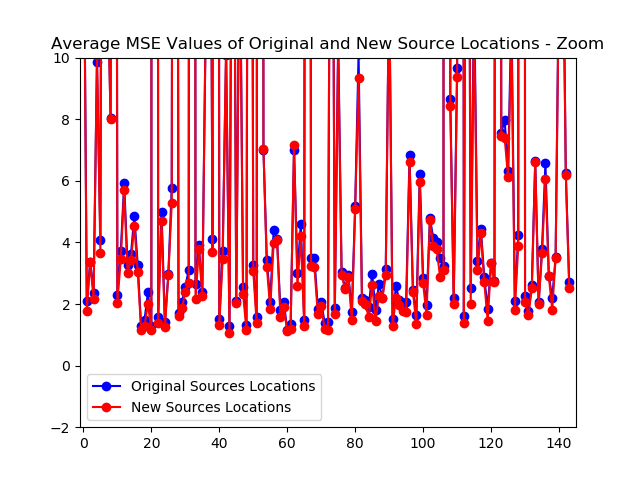
\includegraphics[scale=0.5]{figures/ch_7/M_N_1.png}
	\caption{MSE for system with $\frac{1}{3} M<N$}
	\label{fig:M_N_1}
\end{figure}  
\begin{itemize}
\item  here we have removed $\frac{1}{3}$ of the sensors. The aim is to see if we still can recover the same sources. 
\item plot \ref{fig:M_N_1} is the MSE for every segment, this is to be compared the first plot. It is seen that ...
\item plot \ref{fig:M_N_3} is the MSE of one segment 
\item plot \ref{fig:M_N_2} show an example of the recovered sources for one segment, maybe only few sources should be plotted for better visualisation
\end{itemize}
\begin{figure}[H]
    \centering
	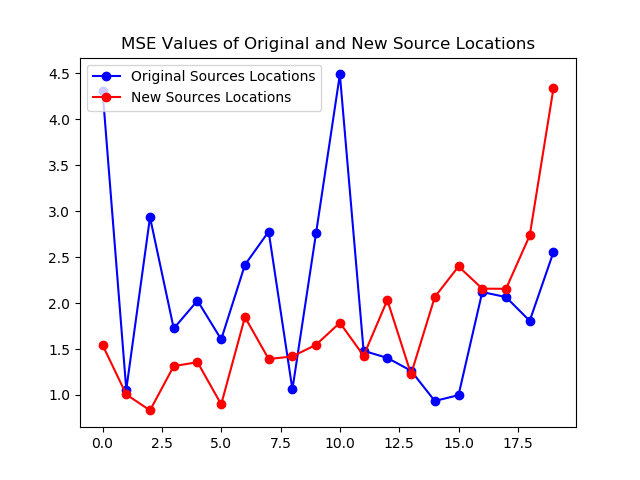
\includegraphics[scale=0.5]{figures/ch_7/M_N_3.png}
	\caption{MSE of one segment of the system with $\frac{1}{3} M<N$}
	\label{fig:M_N_3}
\end{figure}
\begin{figure}[H]
    \centering
	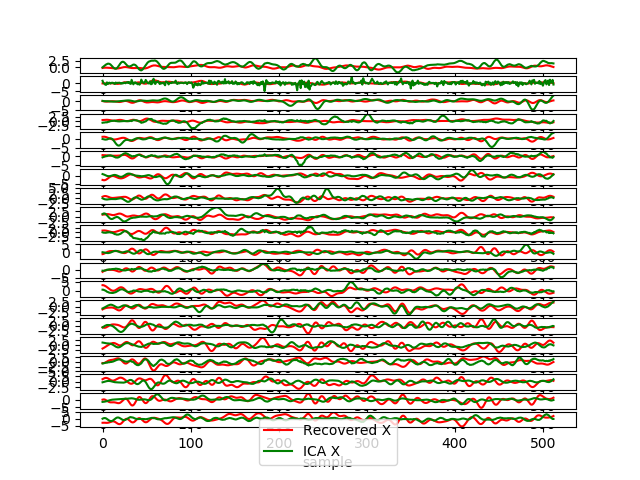
\includegraphics[scale=0.5]{figures/ch_7/M_N_2.png}
	\caption{example of one segment of the system with $\frac{1}{3} M<N$}
	\label{fig:M_N_2}
\end{figure}  



\subsection{Test with $\frac{1}{2} M<N$ on EEG Data Set}
\begin{figure}[H]
    \centering
	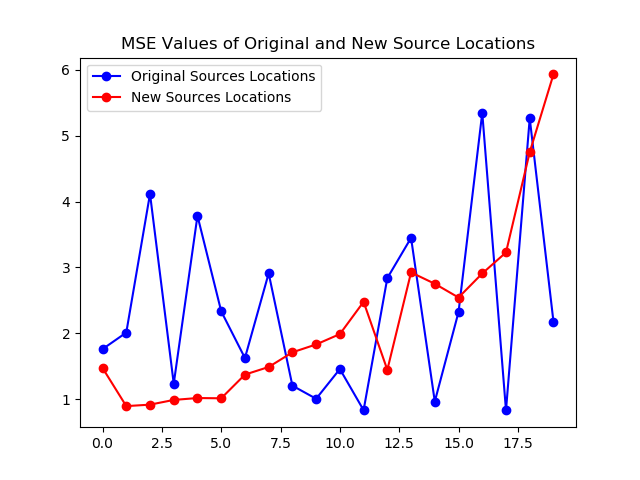
\includegraphics[scale=0.5]{figures/ch_7/M__N_1.png}
	\caption{MSE for system with $\frac{1}{3} M<N$}
	\label{fig:M__N_1}
\end{figure}  
\begin{itemize}
\item  here we have removed $\frac{1}{3}$ of the sensors. The aim is to see if we still can recover the same sources. 
\item plot \ref{fig:M__N_1} is the MSE for every segment, this is to be compared the first plot. It is seen that ...
\item plot \ref{fig:M__N_3} is the MSE of one segment 
\item plot \ref{fig:M__N_2} show an example of the recovered sources for one segment, maybe only few sources should be plotted for better visualisation
\end{itemize}
\begin{figure}[H]
    \centering
	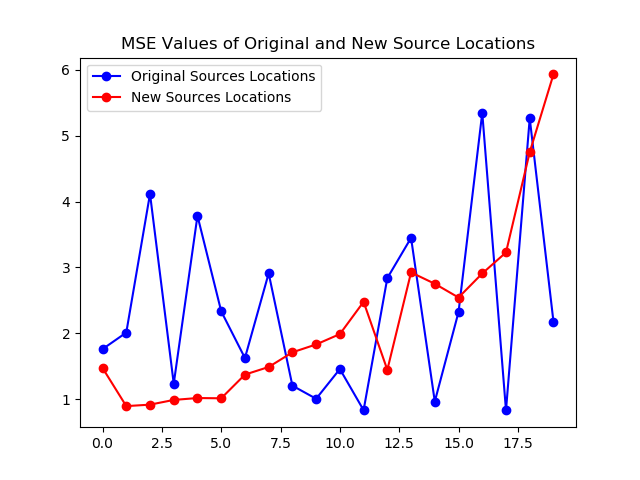
\includegraphics[scale=0.5]{figures/ch_7/M__N_3.png}
	\caption{MSE of one segment of the system with $\frac{1}{3} M<N$}
	\label{fig:M_N_3}
\end{figure}
\begin{figure}[H]
    \centering
	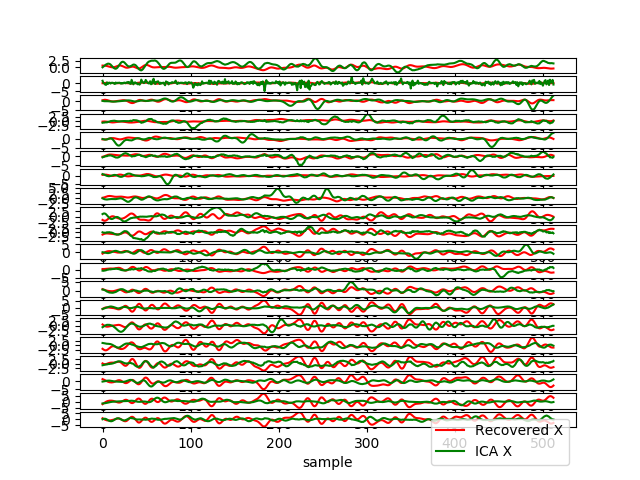
\includegraphics[scale=0.5]{figures/ch_7/M__N_2.png}
	\caption{example of one segment of the system with $\frac{1}{3} M<N$}
	\label{fig:M<N_2}
\end{figure} 